\documentclass[a4paper]{article}
\usepackage{amsmath}
\usepackage{geometry}
\usepackage{float}
\geometry{a4paper, left=2.54cm, right=2.54cm, top=2.54cm, bottom=2.54cm}
\usepackage{indentfirst}
\usepackage{enumitem}
\usepackage{bm}
% 段落間距  (begin doc 才設定)
\usepackage{parskip}
    % 普通文字,行距
    \usepackage[onehalfspacing]{setspace}
    
\usepackage{tabularx}

\usepackage{fontspec,xltxtra,xunicode}
\usepackage{listings}

\setmainfont{Times New Roman}
\usepackage{xeCJK}
\setCJKmainfont[AutoFakeBold=3]{DFKai-SB} %设置中文字体\XeTeXlinebreaklocale “zh”\XeTeXlinebreakskip = 0pt plus 1pt minus 0.1pt %文章内中文自动换行


\usepackage{minted}
\renewcommand{\theFancyVerbLine}{\sffamily\small\arabic{FancyVerbLine}}
\setminted{
  baselinestretch=1,
  fontsize=\fontsize{10pt}{12pt},
  python3=true,
  style=tango,
  linenos=true,
  xleftmargin=20pt,     % 控制行号距离左侧的距离
  frame = single
}




\usepackage{caption}
\newenvironment{code}{\captionsetup{type=listing, font=large, name=List.}}{}
\captionsetup{font={large}}


\usepackage{titlesec}



\def\Large{\fontsize{18}{20}\selectfont}
\def\huge{\fontsize{26}{10}\selectfont}
\def\Huge{\fontsize{36}{54}\selectfont}

\titleformat{\section}
  {\fontsize{18pt}{15}\bfseries}
  {\selectfont\thesection.}
  {0.5em}
  {}

  \titleformat{\subsection}
  {\fontsize{16pt}{15}\bfseries}
  {\selectfont\thesubsection.}
  {0.5em}
  {}

\usepackage{longtable}
\usepackage{array}
\renewcommand{\arraystretch}{1.2}

\renewcommand{\figurename}{Fig.}


\title{\textbf{{\huge Code - HW5} \\ 記憶體積體電路\ Memory\ Circuit\ Design}}
\author{{\Large\textbf{ 電機4A\quad 109501201\quad 陳緯亭}}}
\date{\Large{\today}} 

\begin{document}

\newcolumntype{L}[1]{>{\raggedright\let\newline\\\arraybackslash\hspace{0pt}}m{#1}}
\newcolumntype{C}[1]{>{\centering\let\newline\\\arraybackslash\hspace{0pt}}m{#1}}
\newcolumntype{R}[1]{>{\raggedleft\let\newline\\\arraybackslash\hspace{0pt}}m{#1}}


\maketitle

\fontsize{14pt}{1em}

\selectfont

\begin{figure}[H]
  \centering
  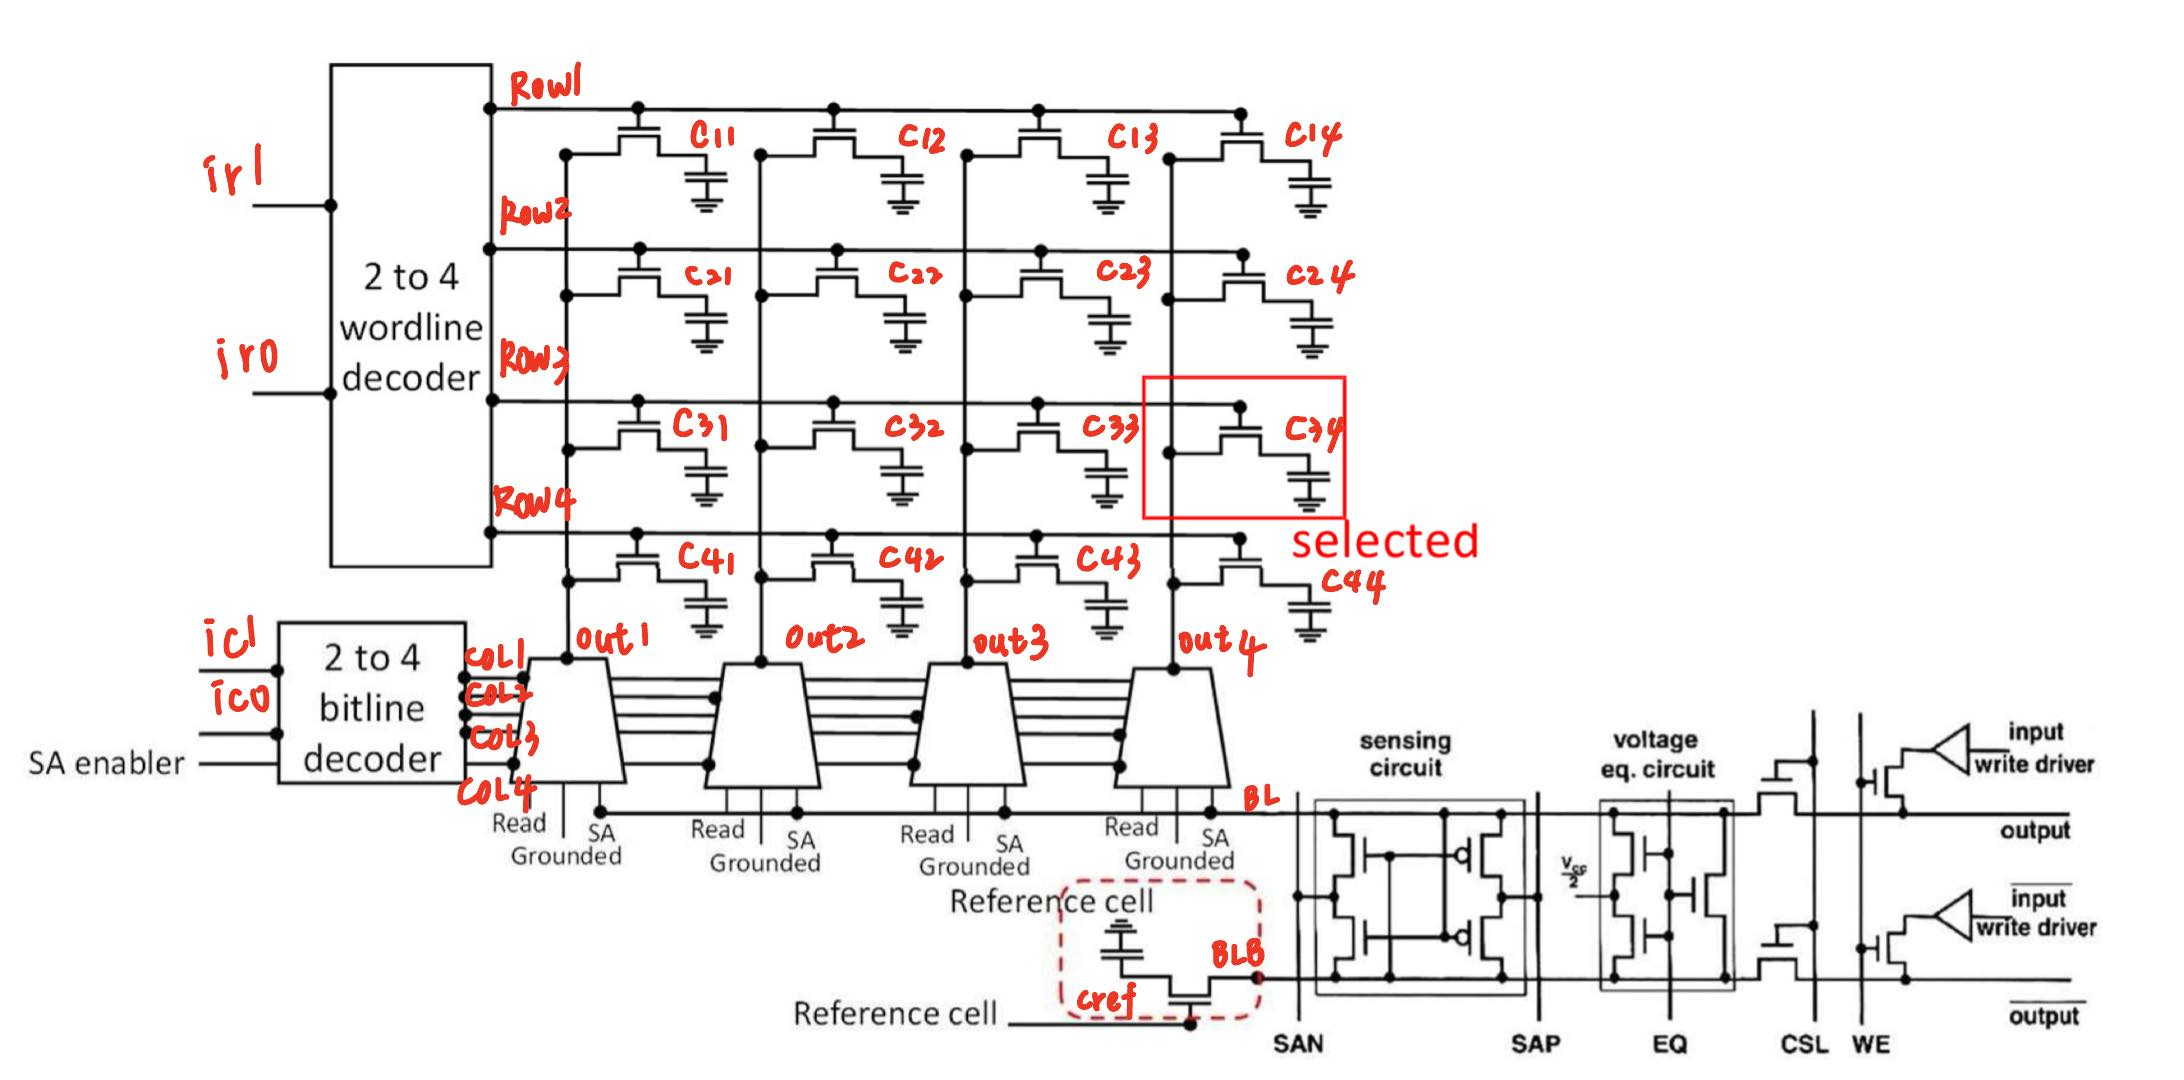
\includegraphics[width = \linewidth]{./img/2023-12-24-17-38-37.png}
  \caption{4x4 mini 1T1C DRAM array}
  \end{figure}


\begin{code}
  \caption{Main code for 4x4 mini 1T1C DRAM array}
  \label{1}
\inputminted{octave}{/Document/Senior/Memory_Circuit_Design/HW5/DRAM1T1C.sp}
\end{code}



\begin{code}
  \caption{Sub-Circuits}
  \label{2}
\inputminted{octave}{/Document/Senior/Memory_Circuit_Design/HW5/subskt.sp}
\end{code}



\end{document}